\rev{
\section{Technique Discussion}

To give a better overview of all the techniques introduced in section \ref{sec:software} and \ref{sec:hardware}, we give a brief summary in this section to see how these techniques contribute to FPGA based NN accelerator designs. Each technique is judged from two aspects: how it affects hardware design and to which level it relates to NN models. Figure~\ref{fig:summary} shows the summary. 

\begin{figure}[ht]
    \centering
    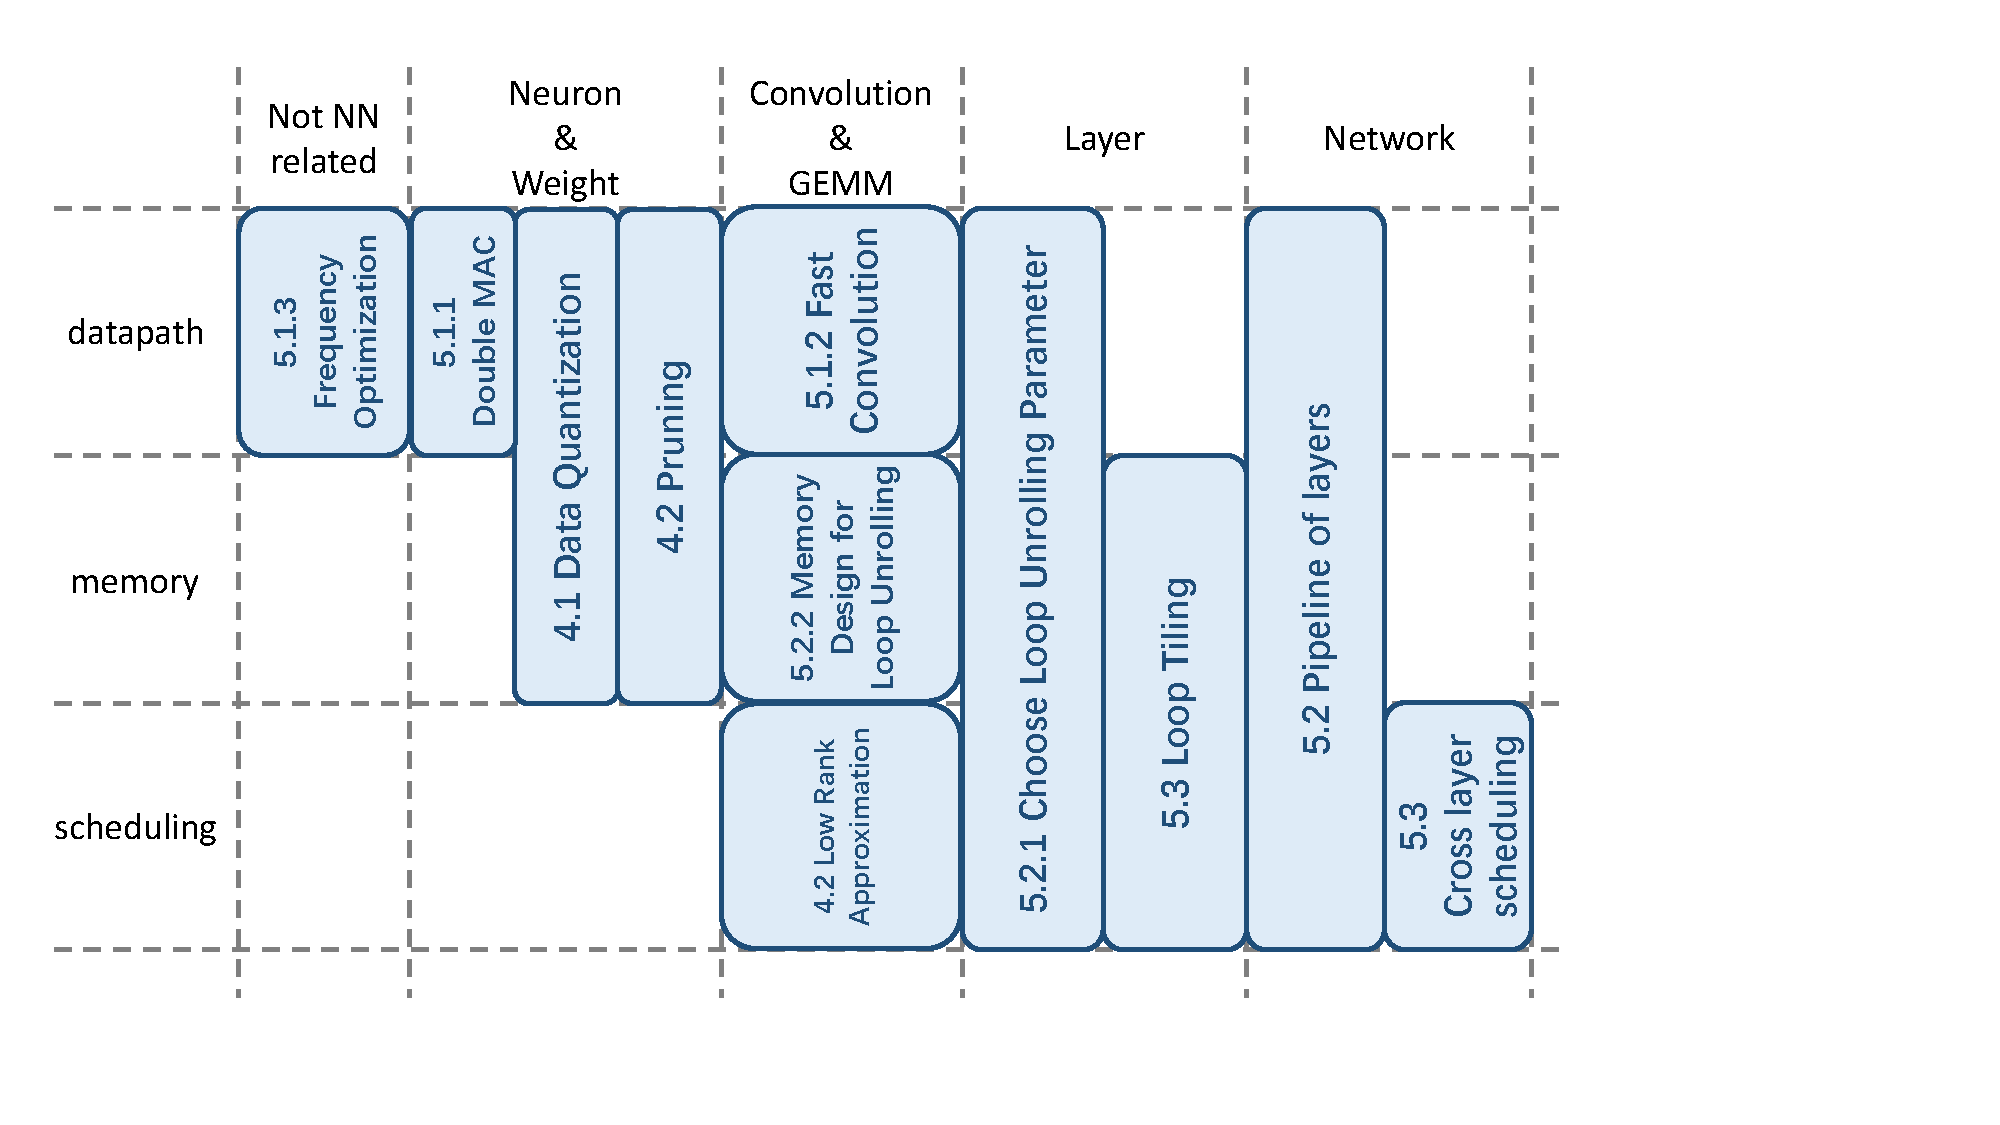
\includegraphics[width=0.8\columnwidth]{fig/summary.pdf}
    \caption{A brief summary of both the software and hardware techniques in section \ref{sec:software} and \ref{sec:hardware}.}
    \label{fig:summary}
\end{figure}

A hardware design basically consists of three parts: datapath, memory, and scheduling. For the design target of high speed, datapath decides the $OPC_{peak}$ while the memory system and scheduling strategy decides $\eta$. For the design target of energy efficiency, datapath decides $E_{op}$ while the memory system decides $N_{SRAM_acc}$ and $N_{DRAM_acc}$. We can see that existing researches are approaching the design target from every aspect by utilizing the neural network model features from single neuron level to the whole network level.

What is the future of FPGA based neural network inference accelerator? Currently, much of the techniques lie in the neuron level and the convolution level. There are two reasons for this. The first reason is that few feature can be utilized in layer level and network level. Most of the existing NN models introduce a simple structure with cascaded layers~\cite{krizhevsky2012imagenet,simonyan2014very} or simply adding a by-path~\cite{he2016deep}. New features like depth-wise convolution~\cite{Howard2017MobileNets} and the complex branch in SSD~\cite{Liu2015SSD} may brings more design opportunities. But few work focuses on these models. The second reason is that the scale of an FPGA chip is limited. An FPGA chip usually consists of hundreds to thousands of DSPs. This number is still too small compared with a single neural network layer with more than 100M operations. 

So further opportunities may come from two aspects. The first is the evolution of network structure. The second is the scaling up of FPGA based system, with larger chips or multiple chips. Existing designs using small models with binary weights are making their FPGAs relatively larger. These designs already introduce some subversive ideas like mapping the whole networks spatially onto hardware~\cite{yang2018fully}. Besides the opportunities, designers are also faced with the scaling up challenges, from the limitation of loop unrolling, bandwidth, etc. 
}